
\chapter{Experimental Validation}
\label{chp:ExpMethodComp}


\section{Segur}
%Wave gauge, conservation properties
%would improved dispersion help
%read other writing on this 
\begin{figure}
	\centering
	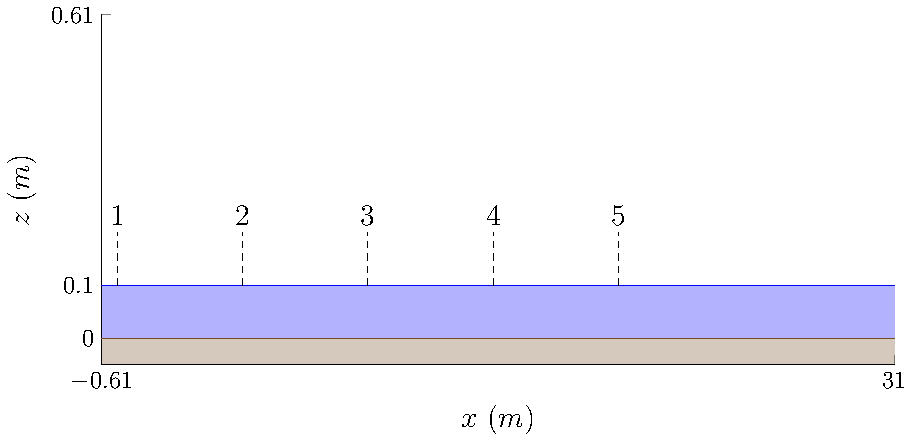
\includegraphics[width=\textwidth]{./chp6/figures/Experiment/Segur/WaveTank.pdf}
	\caption{Diagram demonstrating the water (\squareF{blue}) and the bed (\squareF{brown!80!black}) for the Segur experiments, with the wave gauge locations marked.}
	\label{fig:SegurWT}
\end{figure}

\begin{figure}
	\centering
	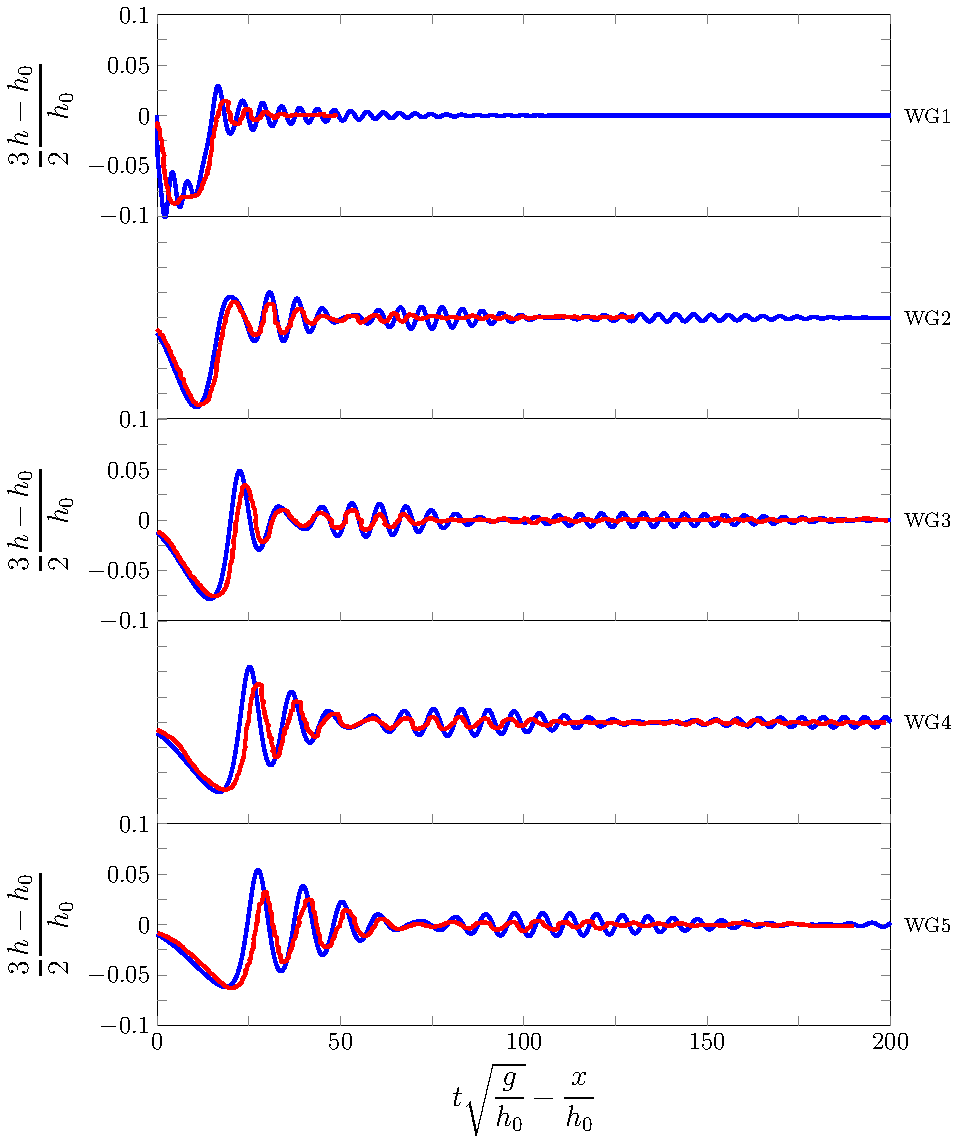
\includegraphics[width=\textwidth]{./chp6/figures/Experiment/Segur/LongWGsFEVM1cm.pdf}
	\caption{FEVM}
	\label{fig:Segur1cmFEVM}
\end{figure}
\begin{figure}
	\centering
	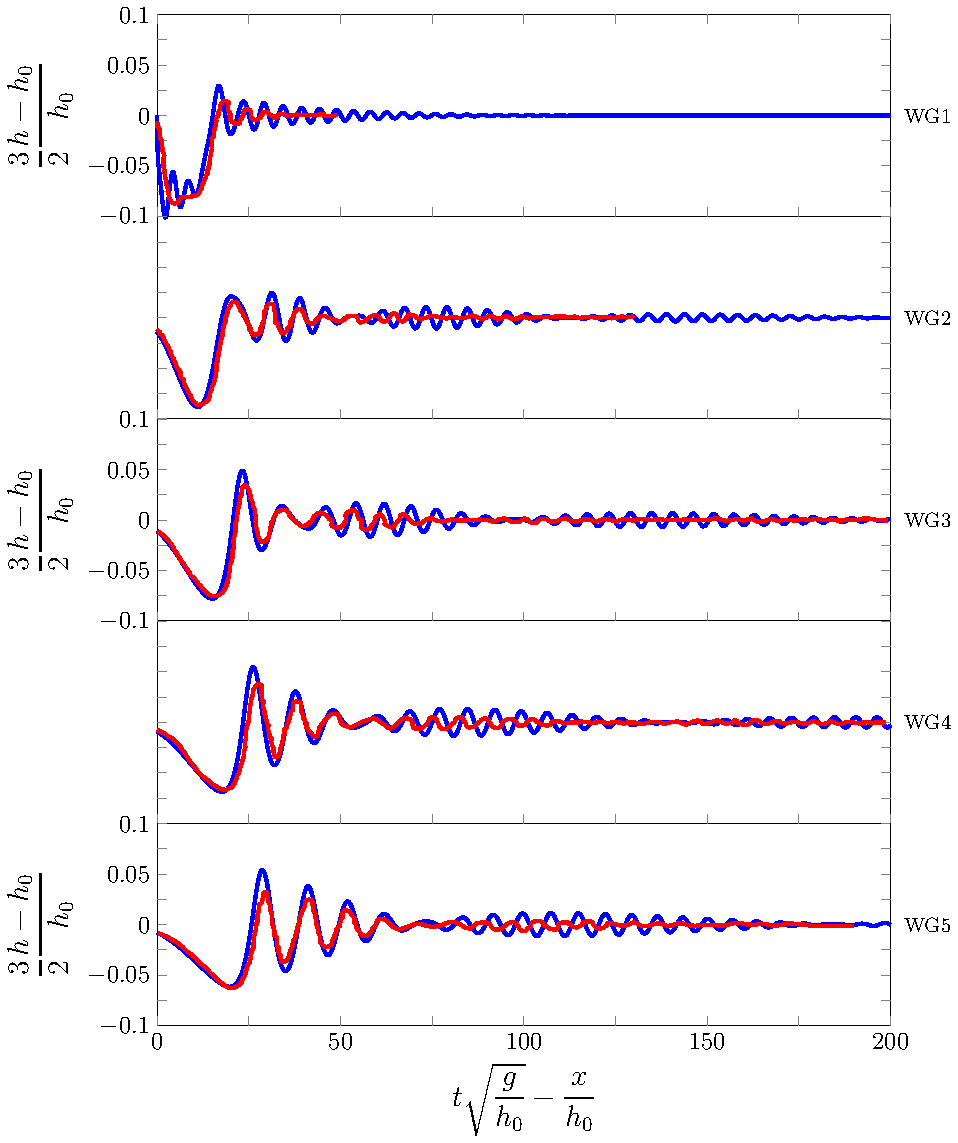
\includegraphics[width=\textwidth]{./chp6/figures/Experiment/Segur/LongWGsFDVM1cm.pdf}
	\caption{FDVM}
	\label{fig:Segur1cmFDVM}
\end{figure}          


\begin{figure}
	\centering
	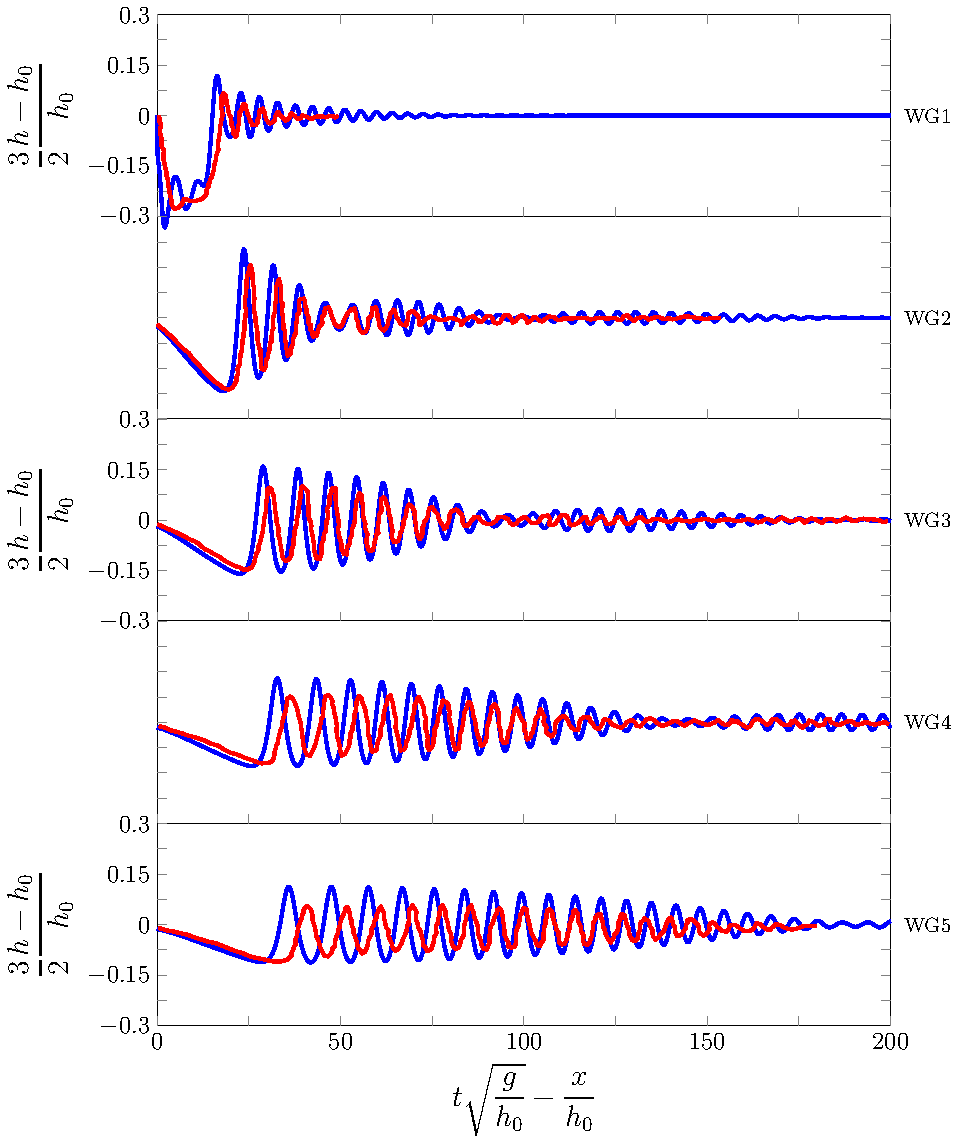
\includegraphics[width=\textwidth]{./chp6/figures/Experiment/Segur/LongWGsFEVM3cm.pdf}
	\caption{FEVM}
	\label{fig:Segur3cmFEVM}
\end{figure}
\begin{figure}
	\centering
	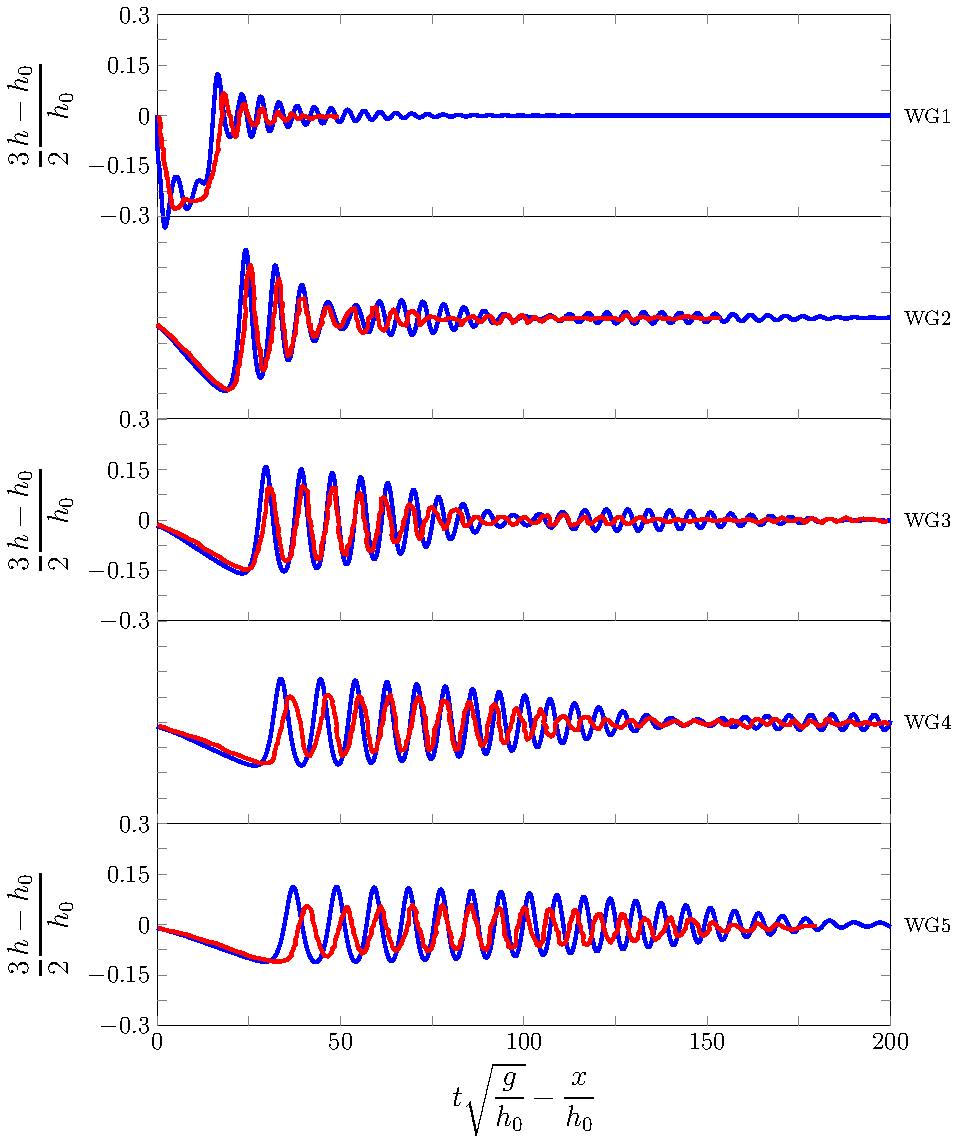
\includegraphics[width=\textwidth]{./chp6/figures/Experiment/Segur/LongWGsFDVM3cm.pdf}
	\caption{FDVM}
	\label{fig:Segur3cmFDVM}
\end{figure}  


\section{Periodic Waves Over A Submerged Bar}
%only pointwise comparison
Beji and Battjes conducted a series of experiments investigating the effect of submerged bars on the propagation of periodic waves \cite{Beji-Battjes-1993-151,Beji-Battjes-1994-1}. The behaviour of these experiments were mainly driven by the dispersion properties of the waves and their interaction with variations in bathymetry. Therefore, these experiments serve as a good benchmark for our numerical schemes abilities to accurately model both the effect of variable bathymetry and dispersive waves. For our purposes we will focus on the monochromatic wave experiments of \citet{Beji-Battjes-1994-1}.

The experiments of \citet{Beji-Battjes-1994-1} were conducted in a wave tank $37.7m$ long, $0.8m$ wide and $0.75m$ high. A diagram of the longitudinal section of the wave tank is given in Figure \ref{fig:BejiWT}. There are seven wave gauges at the following locations; $5.7m$, $10.5m$, $12.5m$, $13.5m$, $14.5m$, $15.7m$ and $17.3m$. Waves are generated from a piston-type wave maker located at $0m$ and travel on the initially still water to the right, over the submerged trapezoidal bar towards a wave absorbing sloped beach.

Two sinusoidal monochromatic non-breaking wave experiments were conducted. A low frequency one with a wavelength $\lambda \approx 3.69m$ and a period of $T = 2s$, and a high frequency one with $\lambda \approx 2.05m$ and a period of $T = 1.25s$. Both experiments had a wave amplitude of $0.01m$ and so both had the same non-linearity parameter $\epsilon = 0.01 / 0.4 = 0.025$. 

We numerically simulated these experiments over the spatial domain $\left[5.7m,150m\right]$ with $\Delta x = 0.1 / 2^4 m$ and $\Delta t = Sp / 2^5$ where $Sp = 0.039$ is the experimental sampling period. These $\Delta x$ and $\Delta t$ values satisfy the CFL condition \eqref{eqn:CFLcond} for these experiments. In our numerical experiments only the submerged trapezoidal bar is present, and the sloping beach is replaced with a very long horizontal bed that ensures that we do not observe any boundary effects in our results.  

To simulate the incoming waves at the upstream boundary we used the first wave gauge as our left boundary condition and used linear extrapolation to calculate the other required $h$ values in the left ghost cell. The velocity boundary conditions were calculated from the height values by solving the continuity equation \eqref{eqn:FullSerreNonConMass} assuming $u$ and $h$ are travelling wave solutions
\begin{equation*}
u(x,t) = \sqrt{g h_0} \; \dfrac{h(x,t) - h_0}{h(x,t)}.
\end{equation*}
Finally the boundary conditions for $G$ were calculated using the boundary conditions for $h$ and $u$. We shall now present our numerical results for the low and high frequency experiments.
%
\begin{figure}
	\centering
		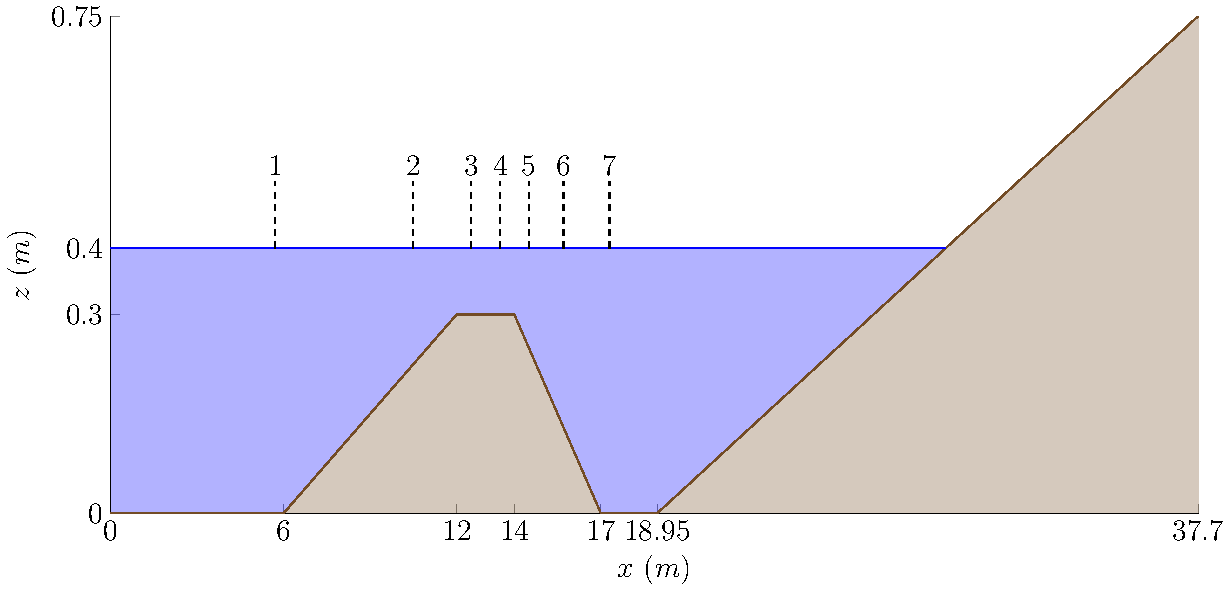
\includegraphics[width=\textwidth]{./chp6/figures/Experiment/Beji/BejiTank.pdf}
	\caption{Diagram demonstrating the water (\squareF{blue}) and the ground  (\squareF{brown!80!black}) for the Beji experiments, with the wave gauge locations marked.}
	\label{fig:BejiWT}
\end{figure}
%
\subsection{Low Frequency Results}
A comparison of wave heights of the experimental and numerical results are located in Figures \ref{fig:BejislWG1to4FEVM} and \ref{fig:BejislWG5to7FEVM} for $\text{FEVM}_2$ and Figures \ref{fig:BejislWG1to4FDVM} and \ref{fig:BejislWG5to7FDVM} for $\text{FDVM}_2$. These numerical schemes both produce identical results for all wave gauges and so this benchmark does not help us discriminate between these two methods. 

These results demonstrate the ability of these numerical methods to recreate the experimental results, particularly for wave gauge $1$ to $5$ where the agreement between experimental and numerical results is best. This validates the numerical schemes for simulating shoaling of dispersion waves as these wave gauges are all located on the windward side of the submerged bar where shoaling occurs in the experiment. 

The numerical results for wave gauges $6$ and $7$ on the leeward side capture some of the wave behaviour but their agreement with the experiments results is much worse. The inadequacy of the numerical results here appears to be due to the discrepancy between the dispersion properties of the Serre equations and water waves, as the numerical solutions of improved dispersion equations \cite{Beji-Battjes-1994-1,Lannes-2013} accurately reproduce the experimental results on the leeward side.

The dispersion of the Serre equations is vital to recreating the experimental results for wave gauges $2$ to $5$, as non-dispersive equations such as the SWWE do a very poor job at simulating this experiment \cite{Pitt-2017-1725}. However, to properly reproduce the experimental results on the leeward side of the slope at wave gauges $6$ and $7$  would require improving the dispersion characteristics of the underlying Serre equations as done by \citet{Barthelemy-2004-315}. Such an improvement can be incorporated into the hybrid FDVM and FEVM numerical methods \cite{Zoppou-2014} but is beyond the scope of this thesis. 

\begin{figure}
	\centering
	\begin{subfigure}{0.5\textwidth}
		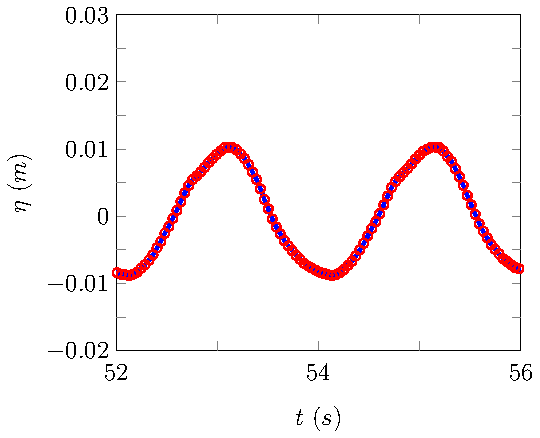
\includegraphics[width=\textwidth]{./chp6/figures/Experiment/Beji/sl/FEVMWG1.pdf}
		\subcaption{Wave Gauge $1$}
		\vspace{0.5cm}
	\end{subfigure}%
	\begin{subfigure}{0.5\textwidth}
		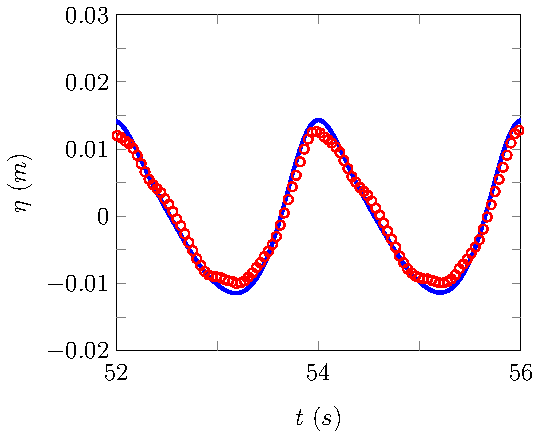
\includegraphics[width=\textwidth]{./chp6/figures/Experiment/Beji/sl/FEVMWG2.pdf}
		\subcaption{Wave Gauge $2$}
		\vspace{0.5cm}
	\end{subfigure}
	\begin{subfigure}{0.5\textwidth}
		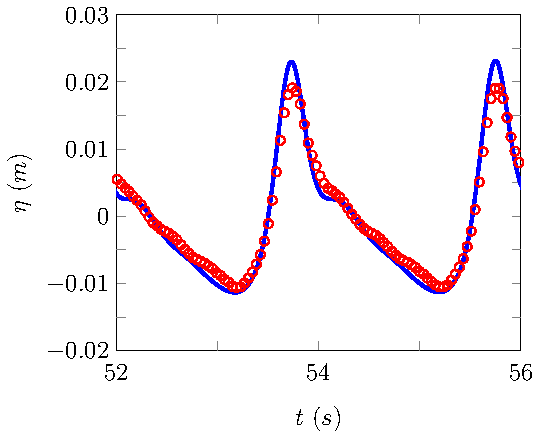
\includegraphics[width=\textwidth]{./chp6/figures/Experiment/Beji/sl/FEVMWG3.pdf}
		\subcaption{Wave Gauge $3$}
		\vspace{0.5cm}
	\end{subfigure}%
	\begin{subfigure}{0.5\textwidth}
		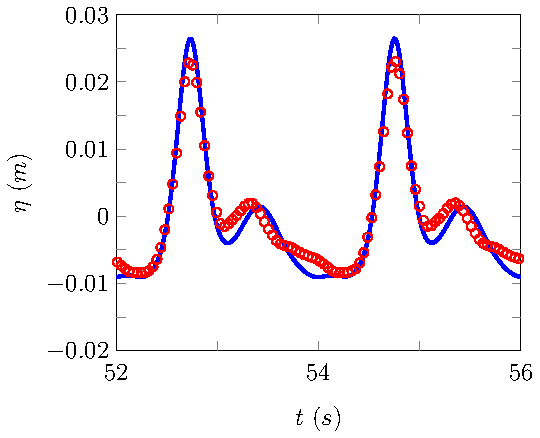
\includegraphics[width=\textwidth]{./chp6/figures/Experiment/Beji/sl/FEVMWG4.pdf}
		\subcaption{Wave Gauge $4$}
		\vspace{0.5cm}
	\end{subfigure}
	\caption{Comparison of the wave heights $\eta$ of the numerical results for the $\text{FEVM}_2$ ({\color{blue}\solidrule}) and the experimental results (\circlet{red}) for wave gauges $1$ - $4$ for the low frequency experiment.}
	\label{fig:BejislWG1to4FEVM}
\end{figure}

\begin{figure}
	\centering
	\begin{subfigure}{0.5\textwidth}
		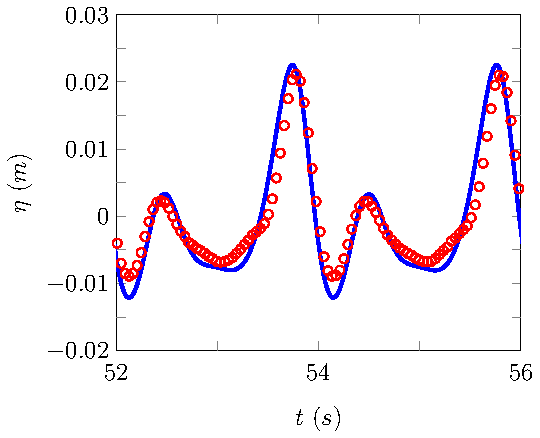
\includegraphics[width=\textwidth]{./chp6/figures/Experiment/Beji/sl/FEVMWG5.pdf}
		\subcaption{Wave Gauge $5$}
		\vspace{0.5cm}
	\end{subfigure}%
	\begin{subfigure}{0.5\textwidth}
		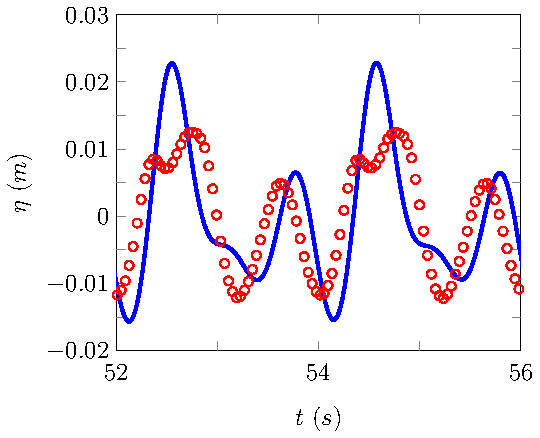
\includegraphics[width=\textwidth]{./chp6/figures/Experiment/Beji/sl/FEVMWG6.pdf}
		\subcaption{Wave Gauge $6$}
		\vspace{0.5cm}
	\end{subfigure}
	\begin{subfigure}{0.5\textwidth}
		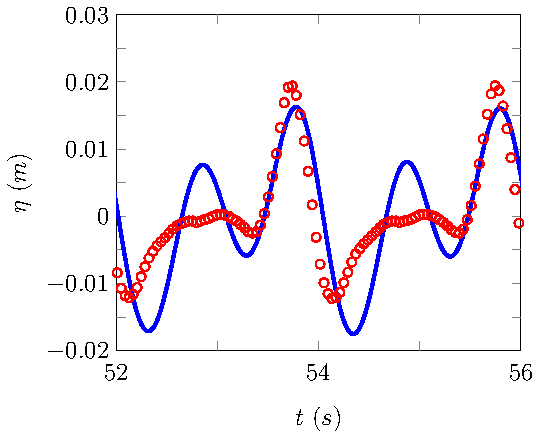
\includegraphics[width=\textwidth]{./chp6/figures/Experiment/Beji/sl/FEVMWG7.pdf}
		\subcaption{Wave Gauge $7$}
		\vspace{0.5cm}
	\end{subfigure}
	\caption{Comparison of the wave heights $\eta$ of the numerical results for the $\text{FEVM}_2$ ({\color{blue}\solidrule}) and the experimental results (\circlet{red}) for wave gauges $5$ - $7$ for the low frequency experiment.}
	\label{fig:BejislWG5to7FEVM}
\end{figure}


\begin{figure}
	\centering
	\begin{subfigure}{0.5\textwidth}
		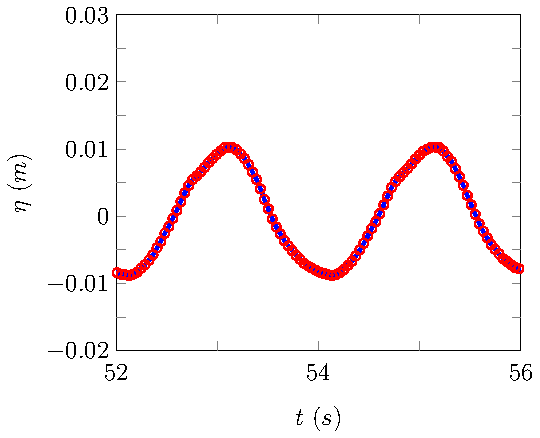
\includegraphics[width=\textwidth]{./chp6/figures/Experiment/Beji/sl/FDVMWG1.pdf}
		\subcaption{Wave Gauge $1$}
		\vspace{0.5cm}
	\end{subfigure}%
	\begin{subfigure}{0.5\textwidth}
		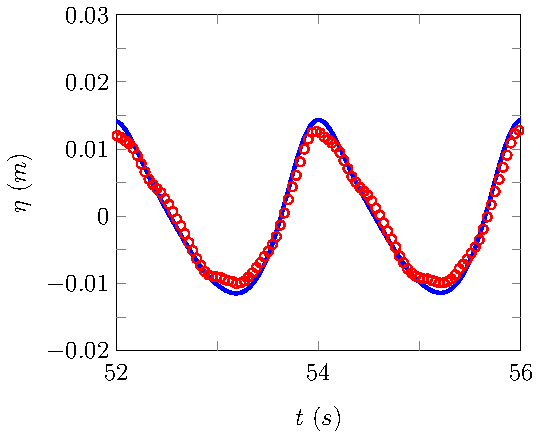
\includegraphics[width=\textwidth]{./chp6/figures/Experiment/Beji/sl/FDVMWG2.pdf}
		\subcaption{Wave Gauge $2$}
		\vspace{0.5cm}
	\end{subfigure}
	\begin{subfigure}{0.5\textwidth}
		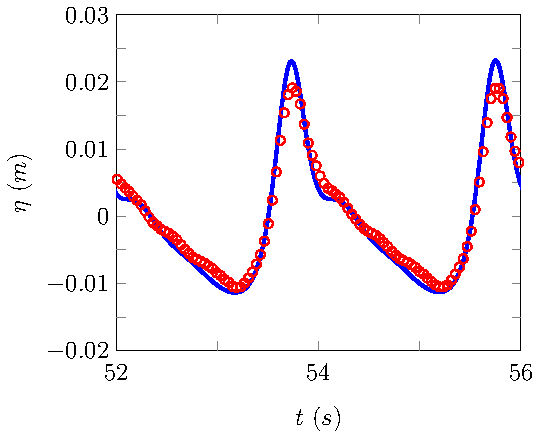
\includegraphics[width=\textwidth]{./chp6/figures/Experiment/Beji/sl/FDVMWG3.pdf}
		\subcaption{Wave Gauge $3$}
		\vspace{0.5cm}
	\end{subfigure}%
	\begin{subfigure}{0.5\textwidth}
		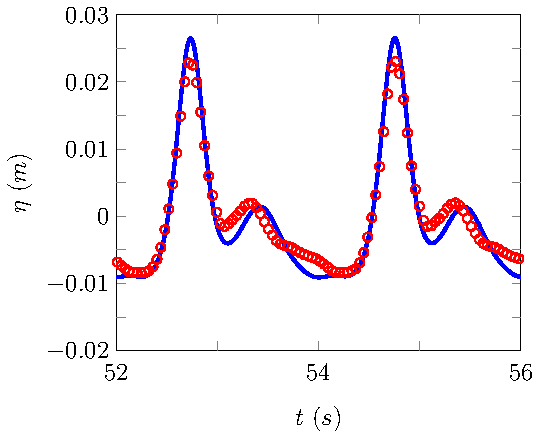
\includegraphics[width=\textwidth]{./chp6/figures/Experiment/Beji/sl/FDVMWG4.pdf}
		\subcaption{Wave Gauge $4$}
		\vspace{0.5cm}
	\end{subfigure}
	\caption{Comparison of the wave heights $\eta$ of the numerical results for the $\text{FDVM}_2$ ({\color{blue}\solidrule}) and the experimental results (\circlet{red}) for wave gauges $1$ - $4$ for the low frequency experiment.}
	\label{fig:BejislWG1to4FDVM}
\end{figure}

\begin{figure}
	\centering
	\begin{subfigure}{0.5\textwidth}
		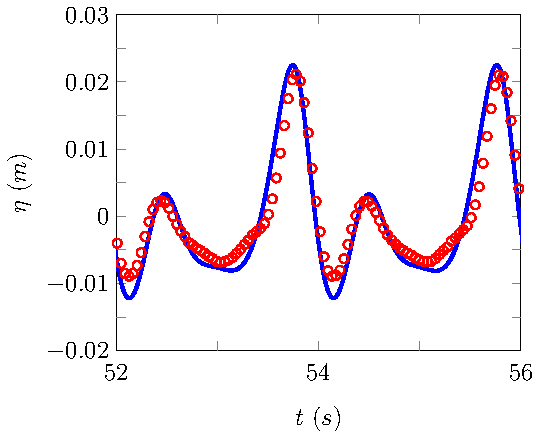
\includegraphics[width=\textwidth]{./chp6/figures/Experiment/Beji/sl/FDVMWG5.pdf}
		\subcaption{Wave Gauge $5$}
		\vspace{0.5cm}
	\end{subfigure}%
	\begin{subfigure}{0.5\textwidth}
		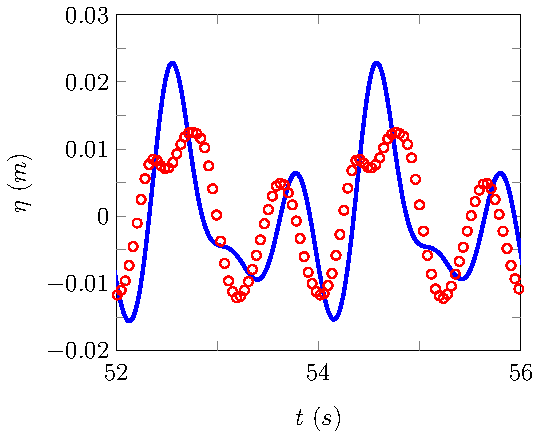
\includegraphics[width=\textwidth]{./chp6/figures/Experiment/Beji/sl/FDVMWG6.pdf}
		\subcaption{Wave Gauge $6$}
		\vspace{0.5cm}
	\end{subfigure}
	\begin{subfigure}{0.5\textwidth}
		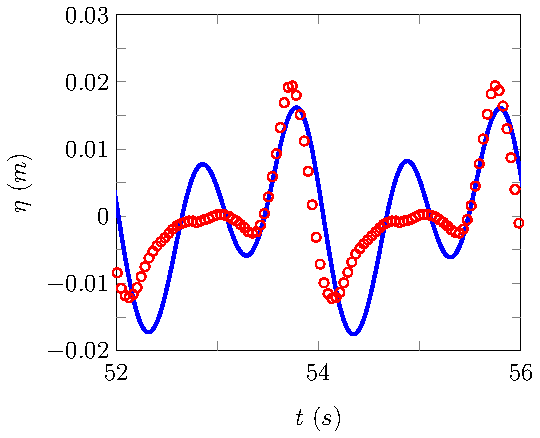
\includegraphics[width=\textwidth]{./chp6/figures/Experiment/Beji/sl/FDVMWG7.pdf}
		\subcaption{Wave Gauge $7$}
		\vspace{0.5cm}
	\end{subfigure}
	\caption{Comparison of the wave heights $\eta$ of the numerical results for the $\text{FDVM}_2$ ({\color{blue}\solidrule}) and the experimental results (\circlet{red}) for wave gauges $5$ - $7$ for the low frequency experiment.}
	\label{fig:BejislWG5to7FDVM}
\end{figure}

\subsection{High Frequency Results}
The wave heights of the experimental and numerical results are given in Figures \ref{fig:BejishWG1to4FEVM} and \ref{fig:BejishWG5to7FEVM} for $\text{FEVM}_2$. While the results for $\text{FDVM}_2$ are given in Figures \ref{fig:BejishWG1to4FDVM} and \ref{fig:BejishWG5to7FDVM}. As for the low frequency experiment, these numerical schemes $\text{FEVM}_2$ and $\text{FDVM}_2$ produce identical results for all wave gauges at this scale and so this benchmark does not discriminate between these two methods. 

As in the low frequency experiment we observe that the numerical results perform well on the windward side of the slope for wave gauges $1$ to $4$ but perform poorly for the leeward side of the slope for wave gauges $5$ to $7$. With the high frequency experiment we see the divergence between the numerical and experimental results earlier than the low frequency experiment, so that now wave gauge 5 which is on the leeward side exhibits a significant difference between the numerical and experimental results. As in the low frequency example improving the dispersion properties of the governing partial differential equations lead to a much better agreement between the numerical and experimental results \cite{Beji-Battjes-1994-1,Lannes-2013}. Because the difference between the dispersion relation of the Serre equations and water waves is largest for higher frequency and therefore for shorter waves \citet{Barthelemy-2004-315} the earlier divergence between experimental and numerical results is expected. 

These numerical results for the $\text{FDVM}_2$ and $\text{FEVM}_2$ agree well with other numerical results for weakly dispersive equations without improved dispersion properties for the simulation of periodic waves over a submerged bar in the literature \cite{Beji-Battjes-1994-1,Lannes-2013,Li-2014-169,Zhang-2013-13}. Therefore, without changing the underlying partial differential equations, our numerical methods as well as these numerical schemes at recreating the experimental results of \citet{Beji-Battjes-1994-1}.

\begin{figure}
	\centering
	\begin{subfigure}{0.5\textwidth}
		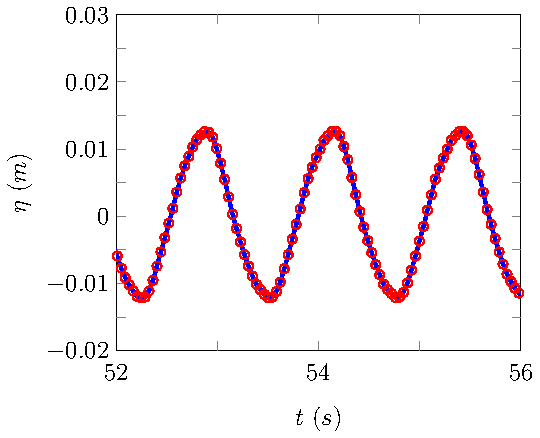
\includegraphics[width=\textwidth]{./chp6/figures/Experiment/Beji/sh/FEVMWG1.pdf}
		\subcaption{Wave Gauge $1$}
		\vspace{0.5cm}
	\end{subfigure}%
	\begin{subfigure}{0.5\textwidth}
		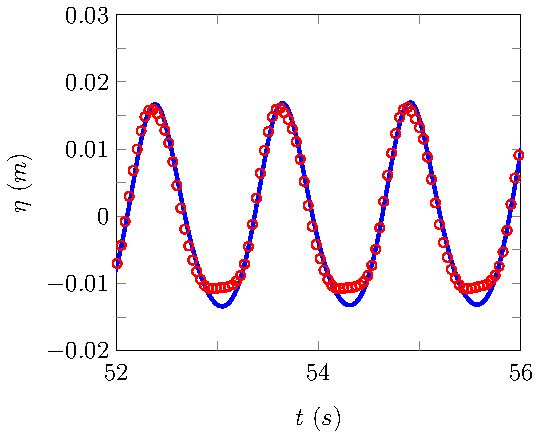
\includegraphics[width=\textwidth]{./chp6/figures/Experiment/Beji/sh/FEVMWG2.pdf}
		\subcaption{Wave Gauge $2$}
		\vspace{0.5cm}
	\end{subfigure}
	\begin{subfigure}{0.5\textwidth}
		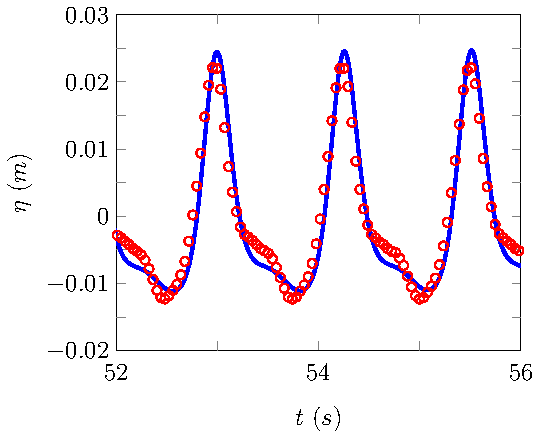
\includegraphics[width=\textwidth]{./chp6/figures/Experiment/Beji/sh/FEVMWG3.pdf}
		\subcaption{Wave Gauge $3$}
		\vspace{0.5cm}
	\end{subfigure}%
	\begin{subfigure}{0.5\textwidth}
		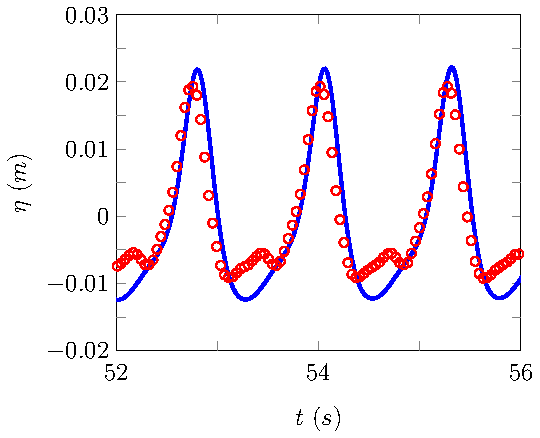
\includegraphics[width=\textwidth]{./chp6/figures/Experiment/Beji/sh/FEVMWG4.pdf}
		\subcaption{Wave Gauge $4$}
		\vspace{0.5cm}
	\end{subfigure}
	\caption{Comparison of the wave heights $\eta$ of the numerical results for the $\text{FEVM}_2$ ({\color{blue}\solidrule}) and the experimental results (\circlet{red}) for wave gauges $1$ - $4$ for the low frequency experiment.}
	\label{fig:BejishWG1to4FEVM}
\end{figure}

\begin{figure}
	\centering
	\begin{subfigure}{0.5\textwidth}
		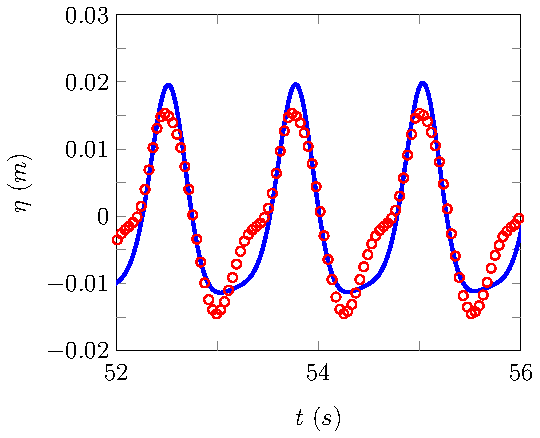
\includegraphics[width=\textwidth]{./chp6/figures/Experiment/Beji/sh/FEVMWG5.pdf}
		\subcaption{Wave Gauge $5$}
		\vspace{0.5cm}
	\end{subfigure}%
	\begin{subfigure}{0.5\textwidth}
		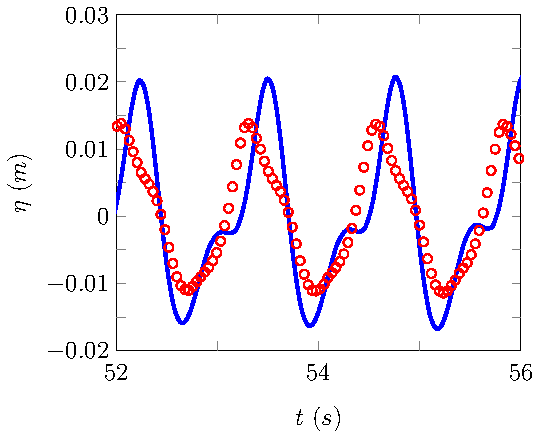
\includegraphics[width=\textwidth]{./chp6/figures/Experiment/Beji/sh/FEVMWG6.pdf}
		\subcaption{Wave Gauge $6$}
		\vspace{0.5cm}
	\end{subfigure}
	\begin{subfigure}{0.5\textwidth}
		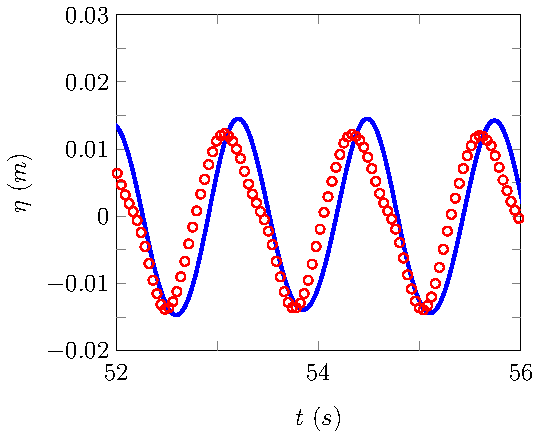
\includegraphics[width=\textwidth]{./chp6/figures/Experiment/Beji/sh/FEVMWG7.pdf}
		\subcaption{Wave Gauge $7$}
		\vspace{0.5cm}
	\end{subfigure}
	\caption{Comparison of the wave heights $\eta$ of the numerical results for the $\text{FEVM}_2$ ({\color{blue}\solidrule}) and the experimental results (\circlet{red}) for wave gauges $5$ - $7$ for the high frequency experiment.}
	\label{fig:BejishWG5to7FEVM}
\end{figure}


\begin{figure}
	\centering
	\begin{subfigure}{0.5\textwidth}
		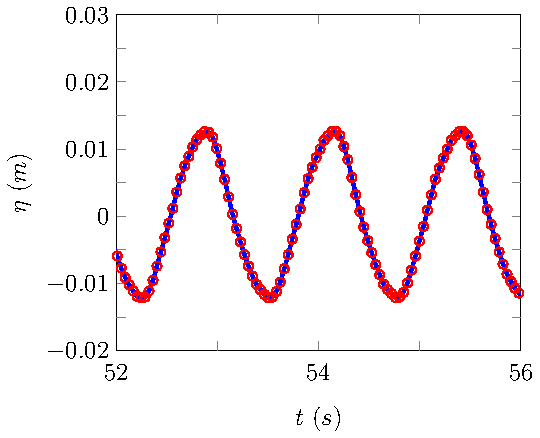
\includegraphics[width=\textwidth]{./chp6/figures/Experiment/Beji/sh/FDVMWG1.pdf}
		\subcaption{Wave Gauge $1$}
		\vspace{0.5cm}
	\end{subfigure}%
	\begin{subfigure}{0.5\textwidth}
		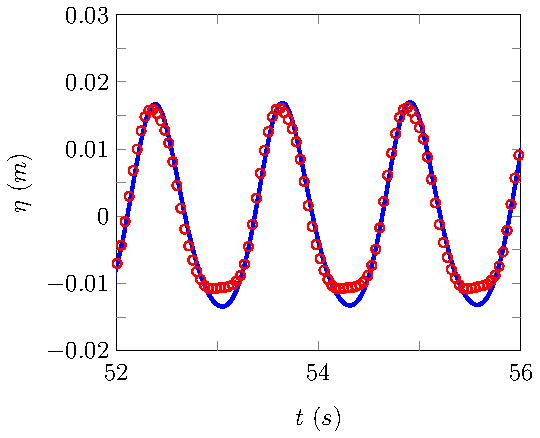
\includegraphics[width=\textwidth]{./chp6/figures/Experiment/Beji/sh/FDVMWG2.pdf}
		\subcaption{Wave Gauge $2$}
		\vspace{0.5cm}
	\end{subfigure}
	\begin{subfigure}{0.5\textwidth}
		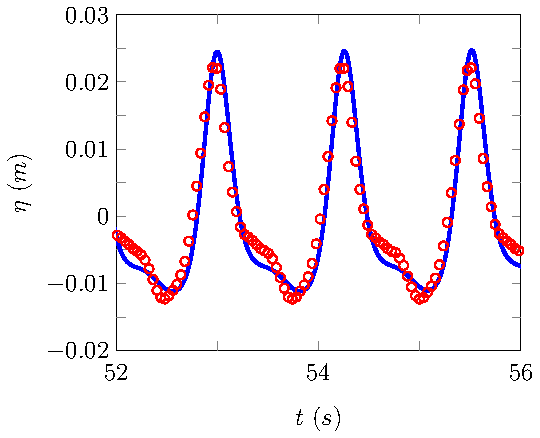
\includegraphics[width=\textwidth]{./chp6/figures/Experiment/Beji/sh/FDVMWG3.pdf}
		\subcaption{Wave Gauge $3$}
		\vspace{0.5cm}
	\end{subfigure}%
	\begin{subfigure}{0.5\textwidth}
		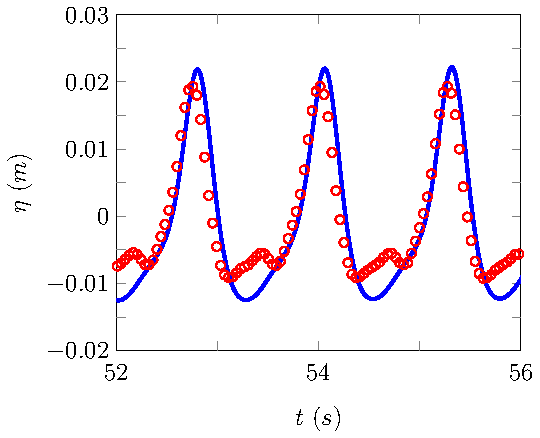
\includegraphics[width=\textwidth]{./chp6/figures/Experiment/Beji/sh/FDVMWG4.pdf}
		\subcaption{Wave Gauge $4$}
		\vspace{0.5cm}
	\end{subfigure}
	\caption{Comparison of the wave heights $\eta$ of the numerical results for the $\text{FDVM}_2$ ({\color{blue}\solidrule}) and the experimental results (\circlet{red}) for wave gauges $1$ - $4$ for the high frequency experiment.}
	\label{fig:BejishWG1to4FDVM}
\end{figure}

\begin{figure}
	\centering
	\begin{subfigure}{0.5\textwidth}
		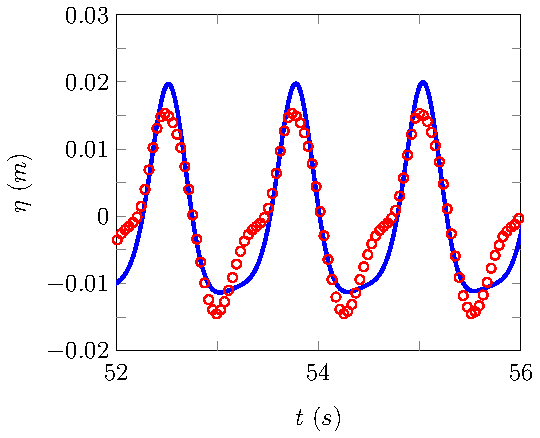
\includegraphics[width=\textwidth]{./chp6/figures/Experiment/Beji/sh/FDVMWG5.pdf}
		\subcaption{Wave Gauge $5$}
		\vspace{0.5cm}
	\end{subfigure}%
	\begin{subfigure}{0.5\textwidth}
		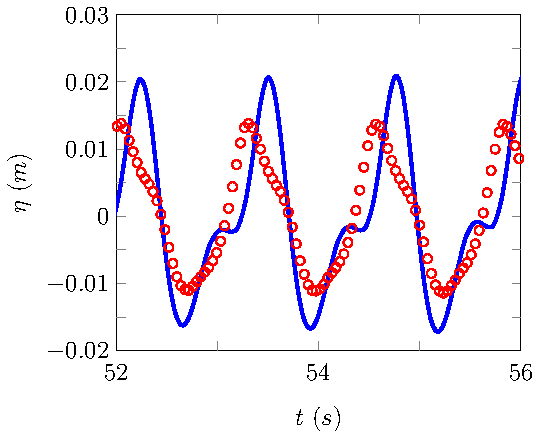
\includegraphics[width=\textwidth]{./chp6/figures/Experiment/Beji/sh/FDVMWG6.pdf}
		\subcaption{Wave Gauge $6$}
		\vspace{0.5cm}
	\end{subfigure}
	\begin{subfigure}{0.5\textwidth}
		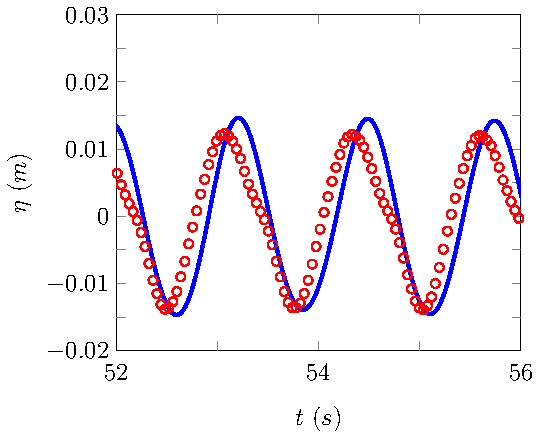
\includegraphics[width=\textwidth]{./chp6/figures/Experiment/Beji/sh/FDVMWG7.pdf}
		\subcaption{Wave Gauge $7$}
		\vspace{0.5cm}
	\end{subfigure}
	\caption{Comparison of the wave heights $\eta$ of the numerical results for the $\text{FDVM}_2$ ({\color{blue}\solidrule}) and the experimental results (\circlet{red}) for wave gauges $5$ - $7$ for the high frequency experiment.}
	\label{fig:BejishWG5to7FDVM}
\end{figure}

\section{Synolakis}
%only pointwise comparison, and H1 and C1 as wave is well defined
%comment on wave breaking number for nonlinearity
\begin{figure}
	\centering
	\begin{subfigure}{0.5\textwidth}
		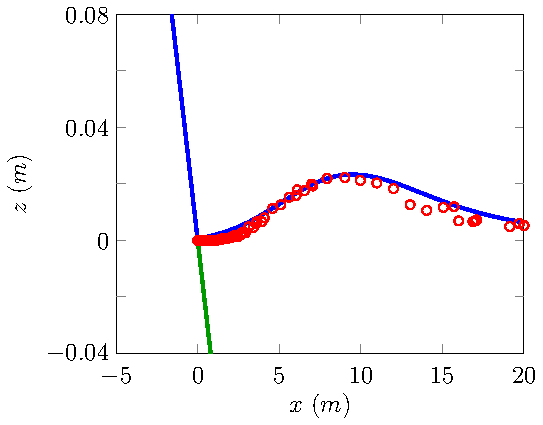
\includegraphics[width=\textwidth]{./chp6/figures/Experiment/Synolakis/H0p0185/FEVM/30s.pdf}
		\subcaption{$t=30s$}
	\end{subfigure}%
	\begin{subfigure}{0.5\textwidth}
		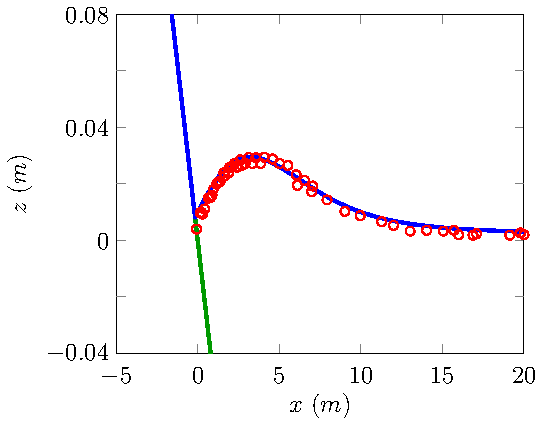
\includegraphics[width=\textwidth]{./chp6/figures/Experiment/Synolakis/H0p0185/FEVM/40s.pdf}
		\subcaption{$t=40s$}
	\end{subfigure}
	\begin{subfigure}{0.5\textwidth}
		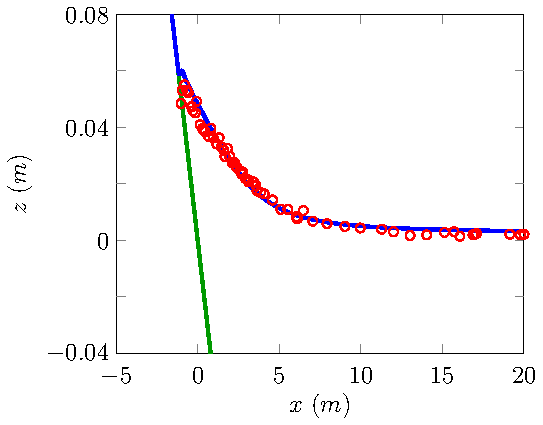
\includegraphics[width=\textwidth]{./chp6/figures/Experiment/Synolakis/H0p0185/FEVM/50s.pdf}
		\subcaption{$t=50s$}
	\end{subfigure}%
	\begin{subfigure}{0.5\textwidth}
		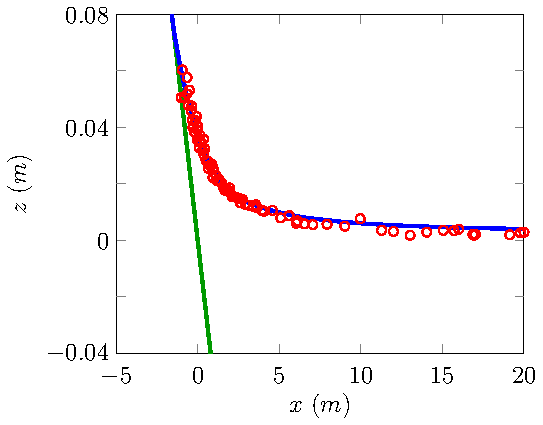
\includegraphics[width=\textwidth]{./chp6/figures/Experiment/Synolakis/H0p0185/FEVM/60s.pdf}
		\subcaption{$t=60s$}
			\end{subfigure}
	\begin{subfigure}{0.5\textwidth}
		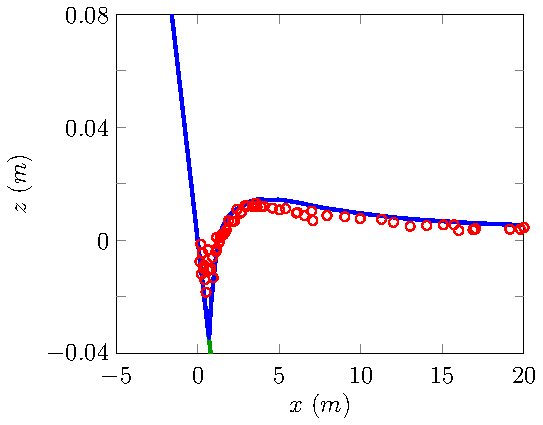
\includegraphics[width=\textwidth]{./chp6/figures/Experiment/Synolakis/H0p0185/FEVM/70s.pdf}
		\subcaption{$t=70s$}
	\end{subfigure}
	\caption{FEVM nonbreak times}
	\label{fig:SynolakisFEVMNoBreak}
\end{figure}

\begin{figure}
	\centering
	\begin{subfigure}{0.5\textwidth}
		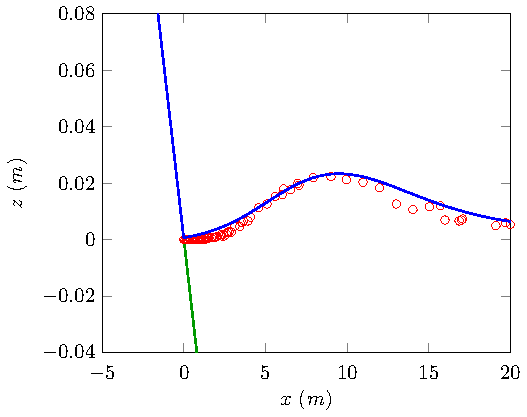
\includegraphics[width=\textwidth]{./chp6/figures/Experiment/Synolakis/H0p0185/FDVM/30s.pdf}
		\subcaption{$t=30s$}
	\end{subfigure}%
	\begin{subfigure}{0.5\textwidth}
		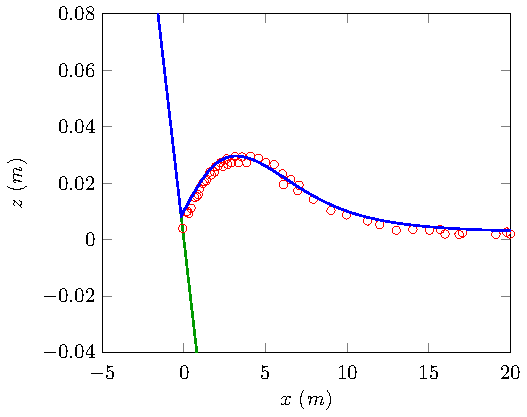
\includegraphics[width=\textwidth]{./chp6/figures/Experiment/Synolakis/H0p0185/FDVM/40s.pdf}
		\subcaption{$t=40s$}
	\end{subfigure}
	\begin{subfigure}{0.5\textwidth}
		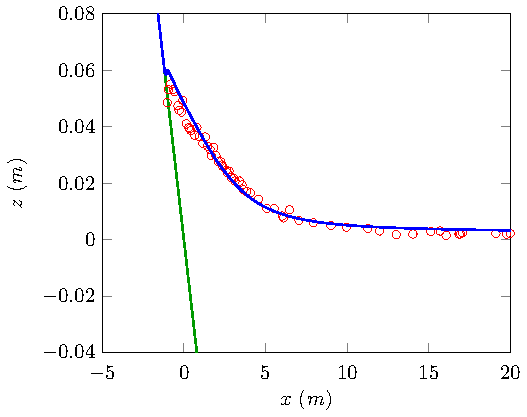
\includegraphics[width=\textwidth]{./chp6/figures/Experiment/Synolakis/H0p0185/FDVM/50s.pdf}
		\subcaption{$t=50s$}
	\end{subfigure}%
	\begin{subfigure}{0.5\textwidth}
		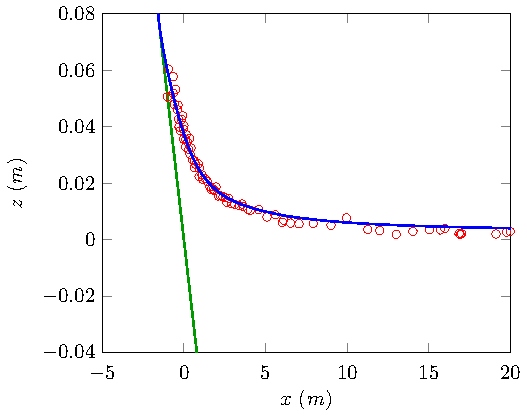
\includegraphics[width=\textwidth]{./chp6/figures/Experiment/Synolakis/H0p0185/FDVM/60s.pdf}
		\subcaption{$t=60s$}
	\end{subfigure}
	\begin{subfigure}{0.5\textwidth}
		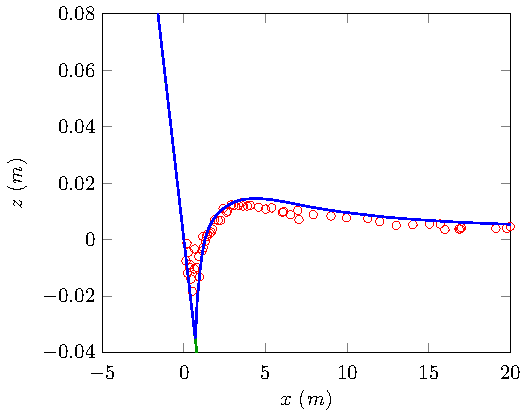
\includegraphics[width=\textwidth]{./chp6/figures/Experiment/Synolakis/H0p0185/FDVM/70s.pdf}
		\subcaption{$t=70s$}
	\end{subfigure}
	\caption{FDVM nonbreak times}
	\label{fig:SynolakisFDVMNoBreak}
\end{figure}


\section{Roeber}
%Wave gauge
%way beyond nolinearity paramter
%in fact this wave breaks, leading to large air entrainment

%wave breaking
%>>> 66 / (sqrt(9.81/2.46))
%33.050420197470373
%>>> 64 / (sqrt(9.81/2.46))
%32.048892312698548

%friction damps these trialing waves?


%Fillipine/Roeber also show discrepancy between numerical model and data before the appearance of the reflected waves, assumption about them having the nolinearity speed may be dubious, good agreement with leading wave


\begin{figure}
	\centering
	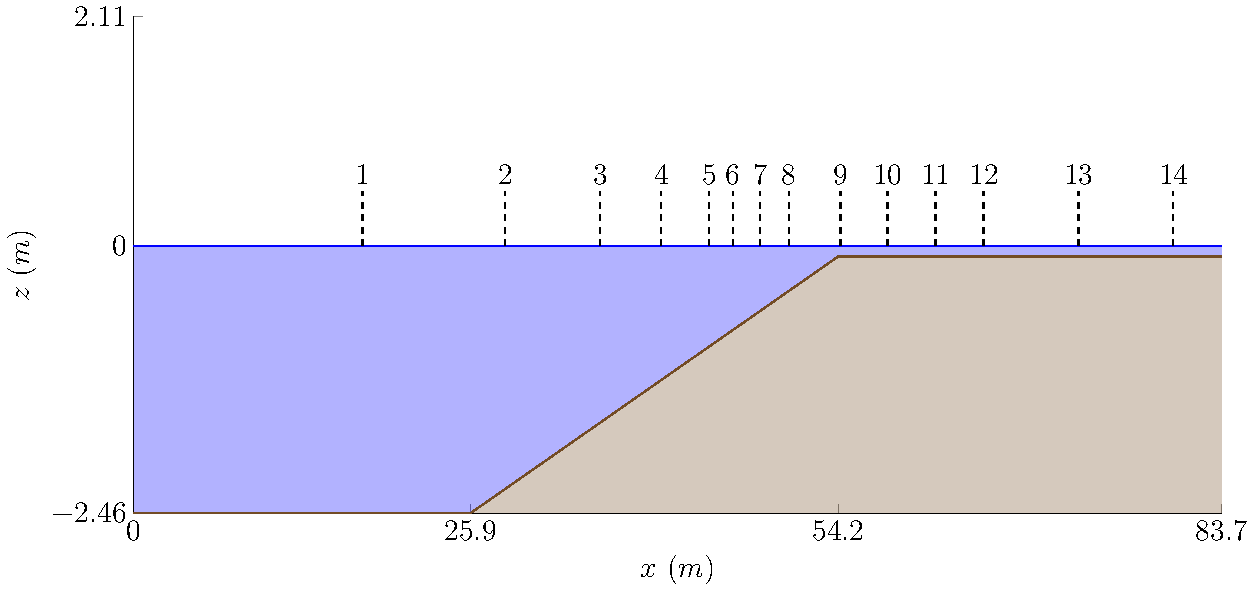
\includegraphics[width=\textwidth]{./chp6/figures/Experiment/Roeber/Trial8/WaveTank.pdf}
	\caption{Diagram demonstrating the water (\squareF{blue}) and the ground  (\squareF{brown!80!black}) for the Beji experiments, with the wave gauge locations marked.}
	\label{fig:RoeberWT}
\end{figure}

\begin{figure}
	\centering
	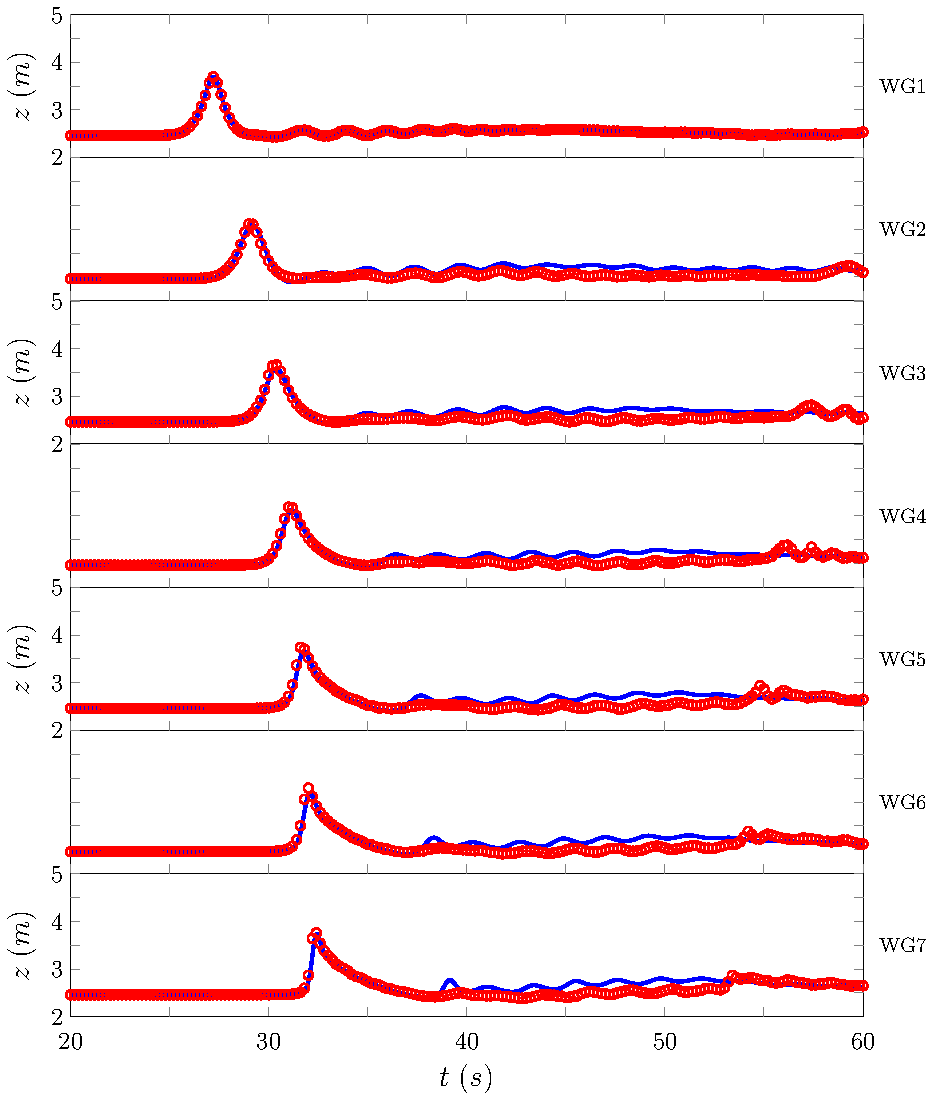
\includegraphics[width=\textwidth]{./chp6/figures/Experiment/Roeber/Trial8/FEVM/LongWGs1.pdf}
	\caption{FEVM}
	\label{fig:Roeber8WG1to7FEVM}
\end{figure}
\begin{figure}
	\centering
	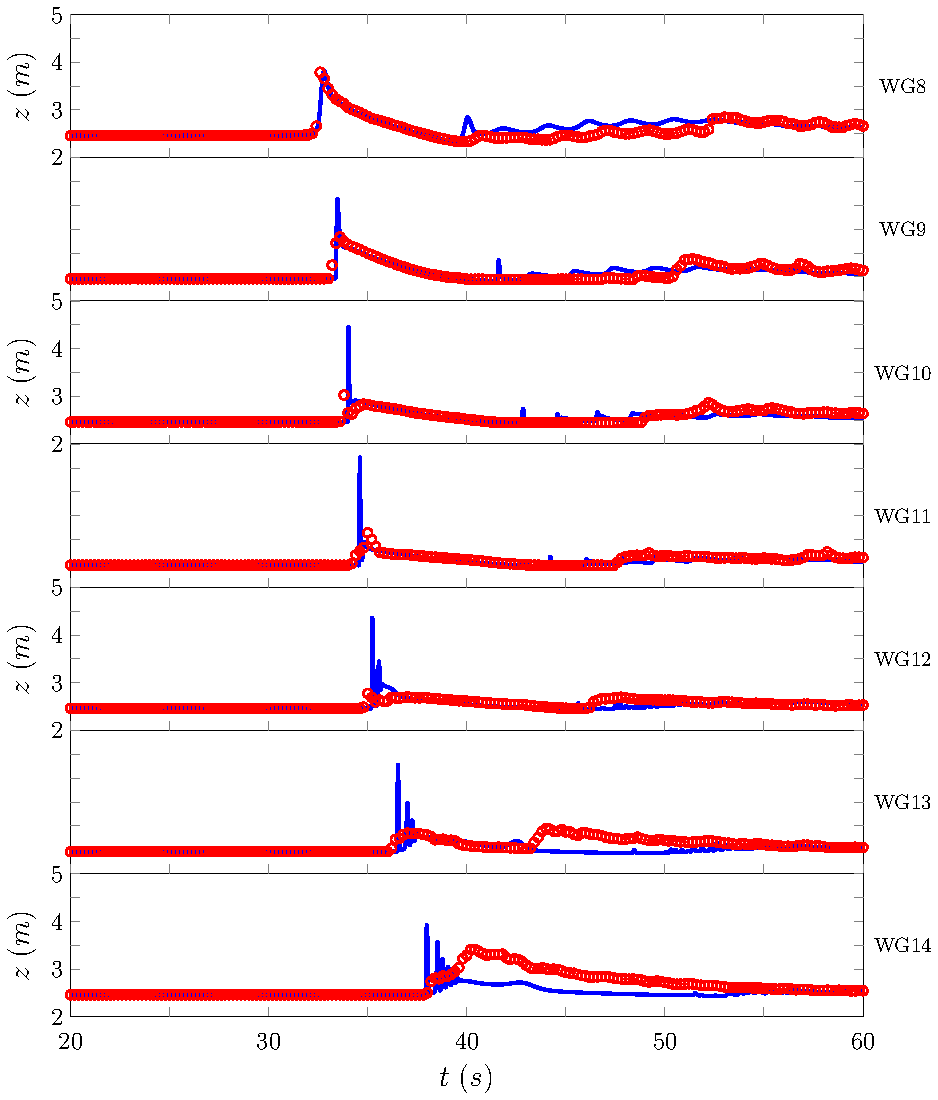
\includegraphics[width=\textwidth]{./chp6/figures/Experiment/Roeber/Trial8/FEVM/LongWGs2.pdf}
	\caption{FEVM}
	\label{fig:Roeber8WG7to14FEVM}
\end{figure}          

\begin{figure}
	\centering
	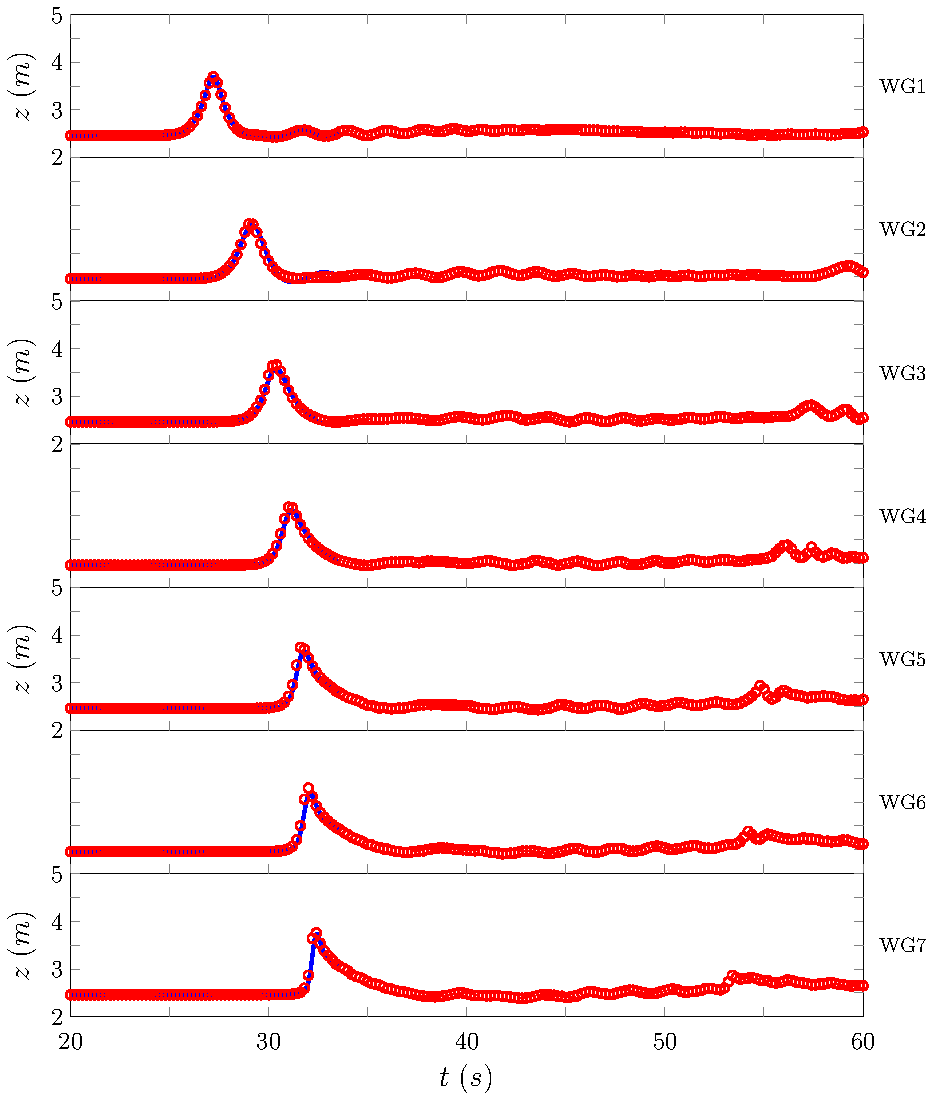
\includegraphics[width=\textwidth]{./chp6/figures/Experiment/Roeber/Trial8/FDVM/LongWGs1.pdf}
	\caption{FEVM}
	\label{fig:Roeber8WG1to7FDVM}
\end{figure}
\begin{figure}
	\centering
	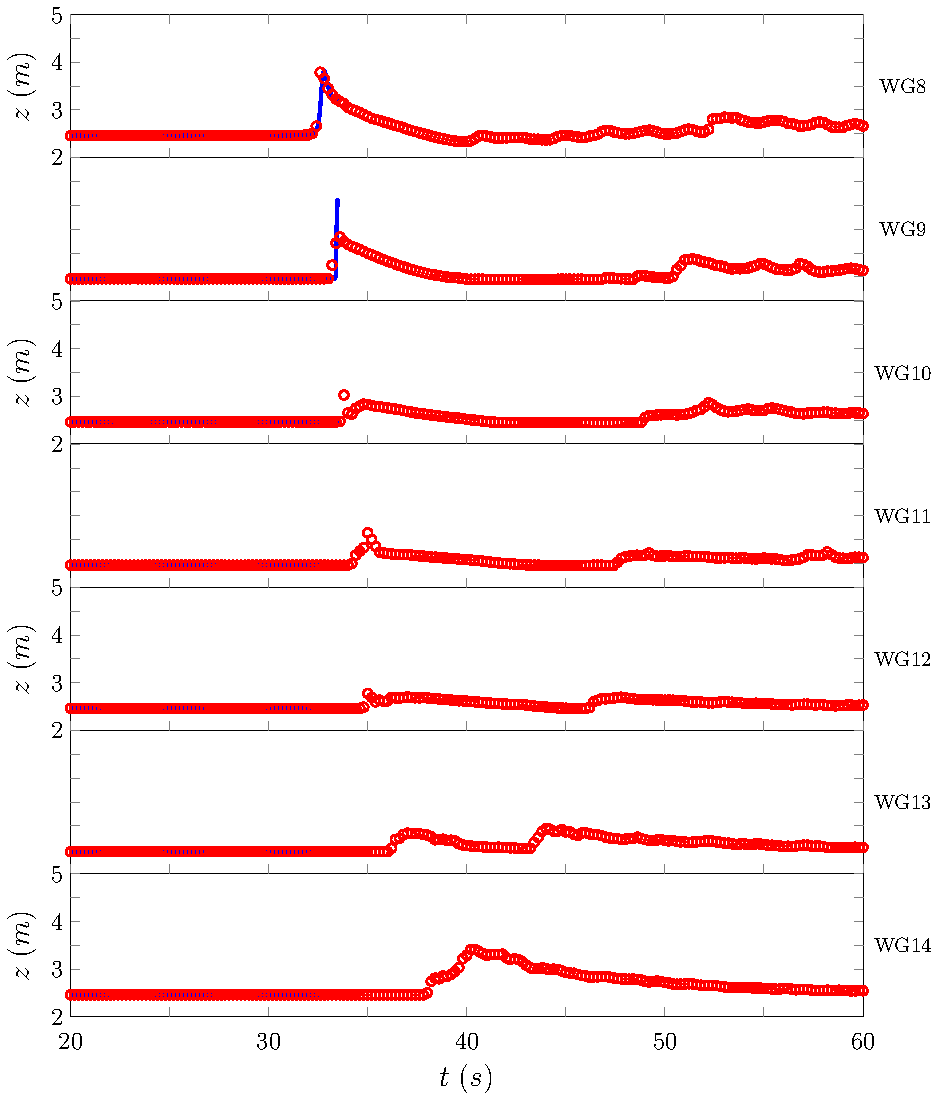
\includegraphics[width=\textwidth]{./chp6/figures/Experiment/Roeber/Trial8/FDVM/LongWGs2.pdf}
	\caption{FEVM}
	\label{fig:Roeber8WG7to14FDVM}
\end{figure} 
